\section{Tree Diagrams and the Multiplication Axiom}\label{section_tree_diagrams}

In this section you will learn to
\begin{enumerate}
    \item Use trees to count possible outcomes in a multi-step process
    \item Use the multiplication axiom to count possible outcomes in a multi-stop process.
\end{enumerate}

In this chapter, we are trying to develop counting techniques that will be used in the next chapter to study probability.  One of the most fundamental of such techniques is called the Multiplication Axiom.  Before we introduce the multiplication axiom, we first look at some examples.

\begin{example}
    If a woman has two blouses and three skirts, how many different outfits consisting of a blouse and a skirt can she wear?
\end{example}

\begin{solution}
    Suppose we call the blouses \( b_1 \) and \( b_2 \), and skirts \( s_1 \), \( s_2 \), and \( s_3 \). We can have the following six outfits: \(b_1s_1\), \(b_1s_2\), \(b_1s_3\), \(b_2s_1\), \(b_2s_2\), \(b_2s_3\)

    Alternatively, we can draw a tree diagram:
    \begin{center}
        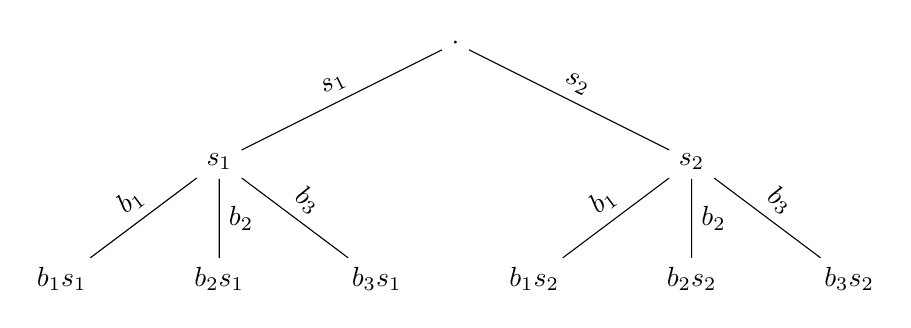
\begin{tikzpicture}[level 1/.style={sibling distance=6cm},
                level 2/.style={sibling distance=2cm}]
            % every node/.style = {shape=rectangle, rounded corners,
            %         draw, align=center,
            %         top color=white, bottom color=blue!20}]]
            \node {$\cdot$}
            child { node {$s_1$}
                    child { node {$b_1s_1$}
                            edge from parent
                            node[sloped, above] {$b_1$}
                        }
                    child { node {$b_2s_1$}
                            edge from parent
                            node[right] {$b_2$}
                        }
                    child { node {$b_3s_1$}
                            edge from parent
                            node[sloped, above] {$b_3$}
                        }
                    edge from parent
                    node[sloped, above] {$s_1$}
                }
            child { node {$s_2$}
                    child { node {$b_1s_2$}
                            edge from parent
                            node[sloped, above] {$b_1$}
                        }
                    child { node {$b_2s_2$}
                            edge from parent
                            node[right] {$b_2$}
                        }
                    child { node {$b_3s_2$}
                            edge from parent
                            node[sloped, above] {$b_3$}
                        }
                    edge from parent
                    node[sloped, above] {$s_2$}
                };
        \end{tikzpicture}
    \end{center}
    The tree diagram gives us all six possibilities.  The method involves two steps.  First the woman chooses a blouse.  She has two choices: blouse one or blouse two.  If she chooses blouse one, she has three skirts to match it with; skirt one, skirt two, or skirt three.  Similarly if she chooses blouse two, she can match it with each of the three skirts, again.  The tree diagram helps us visualize these possibilities.

    The reader should note that the process involves two steps.  For the first step of choosing a blouse, there are two choices, and for each choice of a blouse, there are three choices of choosing a skirt.  So altogether there are $2 \cdot 3 = 6$ possibilities.
\end{solution}

If, in the previous example, we add the shoes to the outfit, we have the following problem.

\begin{example}
    If a woman has two blouses, three skirts, and two pumps, how many different outfits consisting of a blouse, a skirt, and a pair of pumps can she wear?
\end{example}

\begin{solution}
    Suppose we call the blouses $b_1$ and $b_2$, the skirts $s_1$, $s_2$, and $s_3$, and the pumps $p_1$, and $p_2$. The following tree diagram will illustrate all the possible outfits.

    \begin{center}
        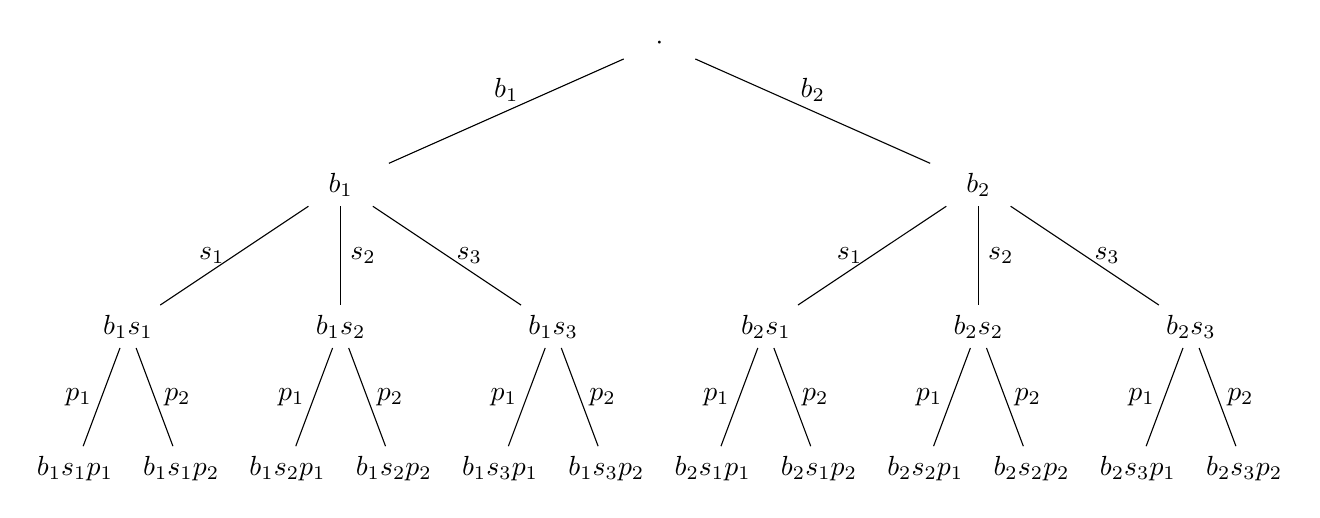
\begin{tikzpicture}[scale=.9]
            \tikzstyle{level 1}=[level distance=2cm, sibling distance=9cm]
            \tikzstyle{level 2}=[level distance=2cm, sibling distance=3cm]
            \tikzstyle{level 3}=[level distance=2cm, sibling distance=1.5cm]
            \tikzstyle{pause} = [text width=4em, text centered]
            \tikzstyle{end} = []

            \node [pause] {$\cdot$}
            child {
                    node [pause] {$b_1$}
                    child {
                            node [pause] {$b_1s_1$}
                            child {
                                    node [end] {$b_1s_1p_1$}
                                    edge from parent
                                    node [left] {$p_1$}
                                }
                            child {
                                    node [end] {$b_1s_1p_2$}
                                    edge from parent
                                    node [right] {$p_2$}
                                }
                            edge from parent
                            node [left] {$s_1$}
                        }
                    child {
                            node [pause] {$b_1s_2$}
                            child {
                                    node [end] {$b_1s_2p_1$}
                                    edge from parent
                                    node [left] {$p_1$}
                                }
                            child {
                                    node [end] {$b_1s_2p_2$}
                                    edge from parent
                                    node [right] {$p_2$}
                                }
                            edge from parent
                            node [right] {$s_2$}
                        }
                    child {
                            node [pause] {$b_1s_3$}
                            child {
                                    node [end] {$b_1s_3p_1$}
                                    edge from parent
                                    node [left] {$p_1$}
                                }
                            child {
                                    node [end] {$b_1s_3p_2$}
                                    edge from parent
                                    node [right] {$p_2$}
                                }
                            edge from parent
                            node [right] {$s_3$}
                        }
                    edge from parent
                    node [above] {$b_1$}
                }
            child {
                    node [pause] {$b_2$}
                    child {
                            node [pause] {$b_2s_1$}
                            child {
                                    node [end] {$b_2s_1p_1$}
                                    edge from parent
                                    node [left] {$p_1$}
                                }
                            child {
                                    node [end] {$b_2s_1p_2$}
                                    edge from parent
                                    node [right] {$p_2$}
                                }
                            edge from parent
                            node [left] {$s_1$}
                        }
                    child {
                            node [pause] {$b_2s_2$}
                            child {
                                    node [end] {$b_2s_2p_1$}
                                    edge from parent
                                    node [left] {$p_1$}
                                }
                            child {
                                    node [end] {$b_2s_2p_2$}
                                    edge from parent
                                    node [right] {$p_2$}
                                }
                            edge from parent
                            node [right] {$s_2$}
                        }
                    child {
                            node [pause] {$b_2s_3$}
                            child {
                                    node [end] {$b_2s_3p_1$}
                                    edge from parent
                                    node [left] {$p_1$}
                                }
                            child {
                                    node [end] {$b_2s_3p_2$}
                                    edge from parent
                                    node [right] {$p_2$}
                                }
                            edge from parent
                            node [right] {$s_3$}
                        }
                    edge from parent
                    node [above] {$b_2$}
                };
        \end{tikzpicture}
    \end{center}

    We count the number of branches in the tree, and see that there are 12 different possibilities.

    This time the method involves three steps. First, the woman chooses a blouse. She has two choices: blouse one or blouse two.  Now suppose she chooses blouse one. This takes us to step two of the process which consists of choosing a skirt. She has three choices for a skirt, and let us suppose she chooses skirt two. Now that she has chosen a blouse and a skirt, we have moved to the third step of choosing a pair of pumps. Since she has two pairs of pumps, she has two choices for the last step. Let us suppose she chooses pumps two. She has chosen the outfit consisting of blouse one, skirt two, and pumps two, or $b_1s_2p_2$. By looking at the different branches on the tree, one can easily see the other possibilities.

    The important thing to observe here, again, is that this is a three step process. There are two choices for the first step of choosing a blouse. For each choice of a blouse, there are three choices of choosing a skirt, and for each combination of a blouse and a skirt, there are two choices of selecting a pair of pumps.

    All in all, we have $2 \cdot 3 \cdot 2 = 12$ different possibilities.
\end{solution}

Tree diagrams help us visualize the different possibilities, but they are not practical when the possibilities are numerous. Besides, we are mostly interested in finding the number of elements in the set and not the actual list of all possibilities; once the problem is envisioned, we can solve it without a tree diagram. The two examples we just solved may have given us a clue to do just that.

Let us now try to solve Example 2 without a tree diagram. The problem involves three steps: choosing a blouse, choosing a skirt, and choosing a pair of pumps. The number of ways of choosing each are listed below. By multiplying these three numbers we get 12, which is what we got when we did the problem using a tree diagram.

\begin{center}
    \begin{tabular}{|c|c|c|}
        \hline
        The number of ways & The number of ways & The number of ways \\
        to choose a blouse & to choose a skirt  & to choose pumps    \\
        \hline
        2                  & 3                  & 2                  \\
        \hline
    \end{tabular}
\end{center}

The procedure we just employed is called the multiplication axiom.

\begin{summarybox}{THE MULTIPLICATION AXIOM}
    If a task can be done in \(m\) ways, and a second task can be done in \(n\) ways, then the operation involving the first task followed by the second can be performed in \(m \cdot n\) ways.
\end{summarybox}

The general multiplication axiom is not limited to just two tasks and can be used for any number of tasks.

\begin{example}
    A truck license plate consists of a letter followed by four digits. How many such license plates are possible?
\end{example}

\begin{solution}
    Since there are 26 letters and 10 digits, we have the following choices for each.
    \[
        \begin{array}{|c|c|c|c|c|}
            \hline
            \text{Letter} & \text{Digit} & \text{Digit} & \text{Digit} & \text{Digit} \\
            \hline
            26            & 10           & 10           & 10           & 10           \\
            \hline
        \end{array}
    \]
    Therefore, the number of possible license plates is \( 26 \cdot 10 \cdot 10 \cdot 10 \cdot 10 = 260000 \).
\end{solution}

\begin{example}
    In how many different ways can a 3-question true-false test be answered?
\end{example}

\begin{solution}
    Since there are two choices for each question, we have
    \[
        \begin{array}{|c|c|c|}
            \hline
            \text{Question 1} & \text{Question 2} & \text{Question 3} \\
            \hline
            2                 & 2                 & 2                 \\
            \hline
        \end{array}
    \]
    Applying the multiplication axiom, we get \( 2 \cdot 2 \cdot 2 = 8 \) different ways.

    We list all eight possibilities: TTT, TTF, TFT, TFF, FTT, FTF, FFT, FFF.

    The reader should note that the first letter in each possibility is the answer corresponding to the first question, the second letter corresponds to the answer to the second question, and so on. For example, TFF, says that the answer to the first question is given as true, and the answers to the second and third questions false.
\end{solution}

\begin{example}
    In how many different ways can four people be seated in a row?
\end{example}

\begin{solution}
    Suppose we put four chairs in a row, and proceed to put four people in these seats. There are four choices for the first chair we choose. Once a person sits down in that chair, there are only three choices for the second chair, and so on. We list as shown below.
    \[
        \begin{array}{|c|c|c|c|}
            4 & 3 & 2 & 1 \\
            \hline
        \end{array}
    \]
    So there are altogether \( 4 \cdot 3 \cdot 2 \cdot 1 = 24 \) different ways.
\end{solution}

\begin{example}\label{example_tree_of_three_letter_sequences}
    How many three-letter word sequences can be formed using the letters \{A, B, C\} if no letter is to be repeated?
\end{example}

\begin{solution}
    The problem is very similar to the previous example. Imagine a child having three building blocks labeled A, B, and C. Suppose he puts these blocks on top of each other to make word sequences. For the first letter he has three choices, namely A, B, or C. Let us suppose he chooses the first letter to be a B, then for the second block which must go on top of the first, he has only two choices: A or C. And for the last letter he has only one choice. We list the choices below.
    \[
        \begin{array}{|c|c|c|}
            3 & 2 & 1 \\
            \hline
        \end{array}
    \]
    Therefore, \( 3 \cdot 2 \cdot 1 = 6 \) different word sequences can be formed.

    \begin{center}
        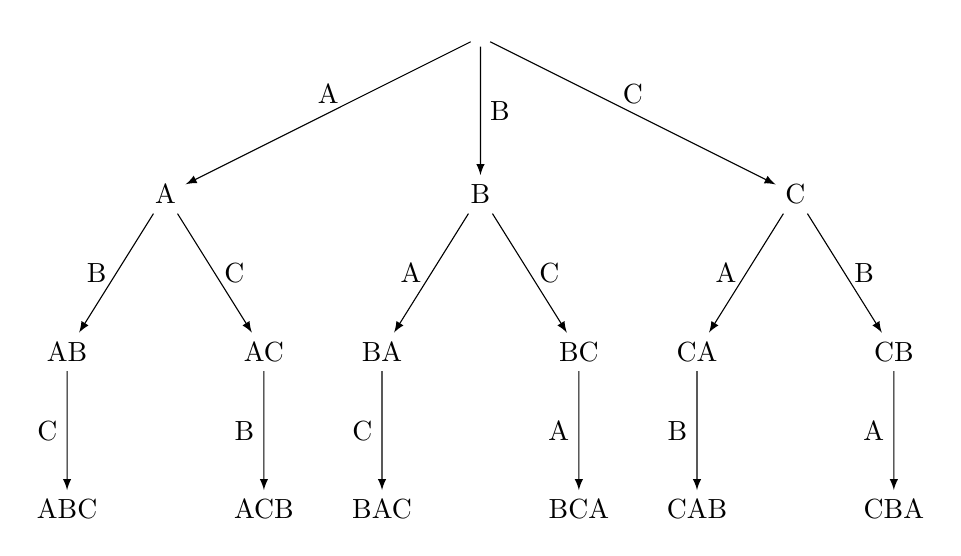
\begin{tikzpicture}[grow=down, edge from parent/.style={draw,-latex}, level distance=1.5cm]
            \tikzstyle{level 1}=[level distance=2cm, sibling distance=4cm]
            \tikzstyle{level 2}=[level distance=2cm, sibling distance=2.5cm]
            \tikzstyle{level 3}=[level distance=2cm, sibling distance=1cm]
            % Root node
            \node {}
            % Level 1
            child {node {A}
                    % Level 2
                    child {node {AB}
                            % Level 3
                            child {node {ABC} edge from parent node[left] {C}
                                }
                            edge from parent node[left] {B}
                        }
                    child {node {AC}
                            child {node {ACB} edge from parent node[left] {B}
                                }
                            edge from parent node[right] {C}
                        }
                    edge from parent node[above] {A}
                }
            child {node {B}
                    child {node {BA}
                            child {node {BAC} edge from parent node[left] {C}
                                }
                            edge from parent node[left] {A}
                        }
                    child {node {BC}
                            child {node {BCA} edge from parent node[left] {A}
                                }
                            edge from parent node[right] {C}
                        }
                    edge from parent node[right] {B}
                }
            child {node {C}
                    child {node {CA}
                            child {node {CAB} edge from parent node[left] {B}
                                }
                            edge from parent node[left] {A}
                        }
                    child {node {CB}
                            child {node {CBA} edge from parent node[left] {A}
                                }
                            edge from parent node[right] {B}
                        }
                    edge from parent node[above] {C}
                };
        \end{tikzpicture}
    \end{center}
\end{solution}

